\section{Precomputing Binary Rank in Blocks}
During our experiment of skewing the tree, we concluded that most of the work during queries is performed inside each node, calculating the binary rank of each bitmap.
It is simply a summing up of popcounts of each word, and we considered whether precomputing these sums for blocks of several words of the bitmaps could improve the query times.

The size of these precomputed blocks is a new variable that could have influence on the running time and memory usage.
Some advantages of larger blocks is less memory usage and fewer precomputed value lookups for the same part of the bitmap.
Some advantages of smaller blocks are that they are more often useful as exemplified by extreme case of a block size equal to the bitmap size which is of little use compared to a block size of half the bitmap size.
The larger block size is only useful for binary rank queries for a position after the halfway point of the bitmap, where the half-size precomputed values can be useful for binary rank queries from $\nicefrac{1}{4}$ into the bitmap.
They can be used from a position at the middle of the block size because the rank can be calculated as the precomputed block value minus the popcount value from the position to the end of the block, which is fewer popcount calculations than calculating popcount from start of bitmap to the queried position. Figure ~\ref{fig:PrecomputePopcountBlock} illustrates this.

\begin{figure}[h]
\caption{Precomputed block value minus the popcount value from the position to the end of the block}
\label{fig:PrecomputePopcountBlock}
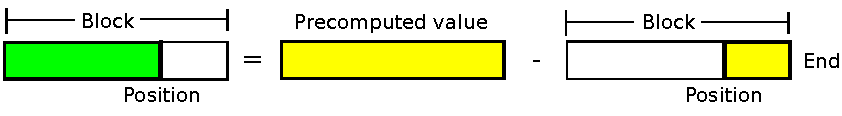
\includegraphics[width=\textwidth]{PrecomputePopcountBlock.pdf}
\end{figure}

Because TLB misses are expensive it could be a great performance improvement to be able to skip entire pages of memory in the queries, and we therefore consider the page size, and multiples of it, good candidates for the block size.

Bitmaps are likely not page-aligned and some might be smaller than the block size, yet we would still like to utilize the precomputed values in these cases.
A way of achieving this would be to concatenate all bitmaps into one giant bitmap for the entire tree and precompute values for each block, keeping them in a seperate vector, and then when needing the binary rank of a area smaller than block size, use the precomputed value and subtract the binary rank of the extra area covered by the block (see figure~\ref{fig:PrecomputePopcountBlock}).
\paragraph{Extra Space Used}~\\
Since each precomputed value cannot exceed the block size in value, assuming we don't use block sizes exceeding $2^{16} = 65536$ bits, we can store them in 16-bit unsigned short integers, which again means, since the page size on our machines are 4096 bits, that we should not use a block size larger than $\frac{65536}{4096} = 16$ pages.

Assuming we store the precomputed values as 16-bit unsigned short integers it will only consume an extra 16 bits per block of which there are $\frac{BitmapSize}{BlockSize}$.
This means, assuming only 1 page per block, an extra space consumption of
\[ \frac{16}{4096} = 0.0039 = 0.39\% \]
of the bitmaps.
Which is even less when considering the total space used including the nodes, and would be less for larger block sizes.

Using one giant bitmap instead of one for each node might also cause a reduction in memory usage from no longer having unused, yet stored, bits at the end of each bitmap.




\subsection{Concatenating the Bitmaps}
We allocate the bitmaps as one giant bitmap the size of the maximum possible size required to store all the bitmaps for all the nodes. The sum of the size of all bitmaps on one layer of the tree can at most be $n$ and we can at most have $h$ layers, so the maximum size becomes
\[n \cdot h\]
where $n$ is the number of characters in the string and $h$ is the max height of the binary wavelet tree which is
\[ h = log(\sigma) \]
We then store an offset and a size for the bitmap in each node, so we can index into the giant bitmap and access the bits corresponding to the node.
After having constructed the entire tree, we then shrink the giant bitmap to fit its actual size, to not waste the memory when the tree is in use for querying. Shrinking the bitmap takes less than a microsecond so it does not impact the construction time in any significant way. We use the \texttt{resize()} and \texttt{shrink\_to\_fit()} vector methods to shrink the bitmap to the size of \texttt{bitmapOffset}, the counter that has been incremented to always point at the next free space in the bitmap during the construction and so is also the actual filled size of the bitmap.
If we had allocated a bitmap for each node individually, they would have been word-aligned, and the bits between the end of one bitmap and the start of another would have gone unused and so, wasted.

Similarly, we allocate a vector for holding the precomputed block values of size
\[ \frac{BitmapSize}{BlockSize} \]
and shrink it afterwards so as not to waste space.

Instead of storing a pointer to the bitmap and precomputed values vector in each node, we store them once for the whole tree and then pass them to the methods that need them.
The nodes now contain, in addition to the previously mentioned pointers, an offset and a size.

\subsection{Experiments}
\subsubsection{Query Running Time for Bitmap with Precomputed Blocks for different Block Sizes}

\subsubsection{Memory Usage of Concatenated vs. Individual Bitmaps}